\section{Manually creating a new \emph{Reprotool} project}

In this section we will walk through the process of creating a new simple \emph{Reprotool} project named \emph{PostOffice}.
Here, we are going to create the project manually. You will not need the project that we are creating here in the later parts
of this documentation. In the next chapters we will deal with importing use-cases into \emph{Reprotool} projects.
All exercises in this documentation will be based on the projects from the following chapters or on the \emph{Reprotool} example projects,
not on the \emph{PostOffice} project from this chapter.

\subsection{\emph{PostOffice} project description}
We will create a simple \emph{PostOffice} project that describes how a letter is written and then taken to the post office.
Our simple project will contain three use-cases and two actors. The \emph{PostOffice} project contains these use-cases:

\begin{enumerate}
 \item {\bf buyEnvelope}
 \item {\bf writeLetter}
 \item {\bf takeLetter}
\end{enumerate}

The \emph{PostOffice} project has these two actors specified:

\begin{enumerate}
 \item {\bf Peter} He writes the letter.
 \item {\bf officer} He works at the post office.
\end{enumerate}

\subsubsection{The \emph{buyEnvelope} use-case}

This use-case has the following structure:

\begin{enumerate}
 \item Peter goes to the shop
 \item Peter stands the queue
 \item Peter buys the envelope
 \item Peter goes home
\end{enumerate}

\subsubsection{The \emph{takeLetter} use-case}
\begin{enumerate}
 \item Peter goes to the post office
 \item Peter stands the queue
 \item Peter becomes impatient

 The queue has more than 10 people:
 \begin{enumerate}
  \item Peter goes home.
 \end{enumerate}


 \item The post officer takes the letter from Peter.
\end{enumerate}


\subsubsection{The \emph{writeLetter} use-case}
\begin{enumerate}

 \item Peter looks at his watches.

    Peter does not have enough free time:
    \begin {enumerate}
      \item Peter does something more important.
    \end {enumerate}

 \item Peter writes the letter.

 \item Peter checks if he has a spare envelope.
    
    Peter does not have a spare envelope:
    \begin {enumerate}
      \item Peter leaves the building.
      \item Include use-case buyEnvelope.
    \end {enumerate}

 \item Peter opens the envelope.

 \item Peter puts the letter into the envelope and closes it.
\end{enumerate}

\subsection{Create a \emph{Reprotool} project}
Create a new \emph{Reprotool} project using the command
\begin{verbatim}
 File / New / Reprotool Project
\end{verbatim}

A \emph{new project} dialog fires up. Enter the project name \emph{postOffice} and press \emph{Enter}. The new \emph{postOffice}
\emph{Reprotool} project has been created. You can view it now in the \emph{Project Explorer}. Now the \emph{project editor} has
started and we can start editing our (now empty) project.

The first thing we are going to do is to add actors to our project. You add actors by clicking the green \emph{plus} sign above the
\emph{Actors} field in the \emph{project editor}. Now please add the two actors to our project.

\subsection{Add use-cases to our project}
Now we are going to add the use-cases to our project. We will describe the process in greater detail for the use-case
\emph{writeLetter}. You add a use-case by clicking the \emph{plus} sign above the Use-cases field of the \emph{Project editor}.
After clicking on the \emph{plus} sign, the \emph{Use-case} editor has started. Now we are going to edit the use-case.

Firstly, enter the use-case name \emph{writeLetter} and think of a suitable \emph{description} of the use-case.
Then select the \emph{Peter} as the \emph{primary actor} of the use-case.

Now it is time to add the individual use-case steps to our use-case. Notice that the use-case by default already contains one single
use-case step. You add other steps by right-clicking on use-case step and select the
\begin{verbatim}
New Sibling / Use Case Step
\end{verbatim}
 command. Now proceed by firstly adding the steps of the \emph{main scenario} only. That is, add the following steps to the use-case:

\begin{enumerate}
 \item Peter looks at his watches.
 \item Peter writes the letter.
 \item Peter checks if he has a spare envelope.
 \item Peter opens the envelope.
 \item Peter puts the letter into the envelope and closes it.
\end{enumerate}

Now we will add an \emph{extension scenario} to the use-case step 1 (Peter looks at his watches). An \emph{extension scenario} is an
ordered set of steps than can be attached to some use-case step. The steps of an extension scenario are executed \emph{after} the execution
of the associated step if the associated condition is met. So now right-click the first use-case step and select this command:
\begin{verbatim}
 New Child / Extensions scenario
\end{verbatim}
A new \emph{extension scenario} has been created. It has the label \emph{1a (ext.)} because it is attached to the use-case step with label
\emph{1}. The created scenario by default contains a single step. Enter this text in the use-case editor right next to the label
\emph{1a (ext.)}
\begin{verbatim}
Peter does not have enough free time:
\end{verbatim}
Then fill the single use-case step of our extension scenario with this text:
\begin{enumerate}
 \item Peter does something more important.
\end{enumerate}

Now create an extension scenario to the step three in a same way. But now attach this text to the extension scenario:
\begin{verbatim}
Peter does not have a spare envelope:
\end{verbatim}

Add a second step to the extension scenario so that it is 2 steps long. And fill the steps with this text:
\begin {enumerate}
 \item Peter leaves the building.
 \item Include use-case buyEnvelope.
\end {enumerate}

Now we are finished with the \emph{writeLetter} use-case. Proceed in a similar way and create the other two missing use-cases.
Select \emph{Peter} as the \emph{primary actor} of the use-case \emph{buyEnvelope} and select the \emph{Officer} as the primary actor
of the \emph{takeLetter} use-case.

In the following figure you can view the \emph{PostOffice} project while editing the \emph{takeLetter} use-case.

\begin{figure}[ht]
  \centering
  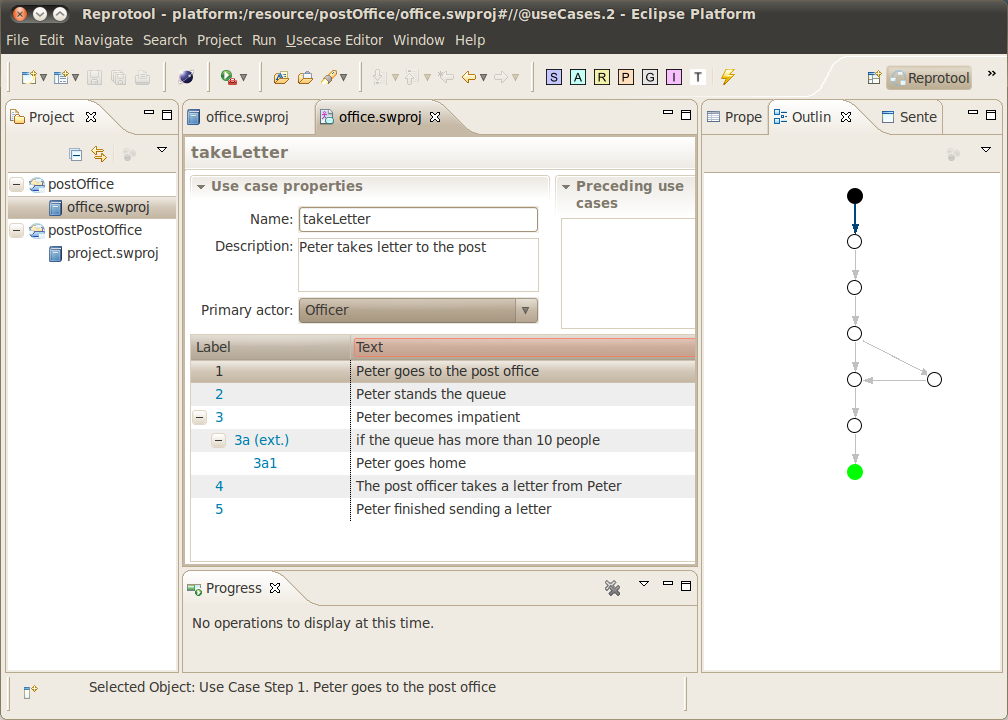
\includegraphics[height=280pt]{images/reprotoolUCEditor}
  \caption{\emph{takeLetter} use-case}
  \label{fig:reprotoolUCEditor}
\end{figure}

\newpage

\subsection{Add \emph{actions} to the use-case steps}

In this step we will need the \emph{Sentence Analysis} view. You can display it by this command:
\begin{verbatim}
 Window / Show View / Other
\end{verbatim}

and select \emph{Reprotool} from the dialog box that appears. Now click on the \emph{Sentence Analysis} and click OK. This should make
the \emph{SentenceAnalysis view} visible.

\subsubsection{\emph{Actions} in the \emph{writeLetter} use-case}

Now we will define the \emph{Abort} action for the only use-case step of the first step extension scenario. Click on the use-case step
with label \emph{1a1} and select \emph{Abort} as \emph{Action Type} in the \emph{Sentence Analysis View}. You can view this situation
in the next picture:

\begin{figure}[ht]
  \centering
  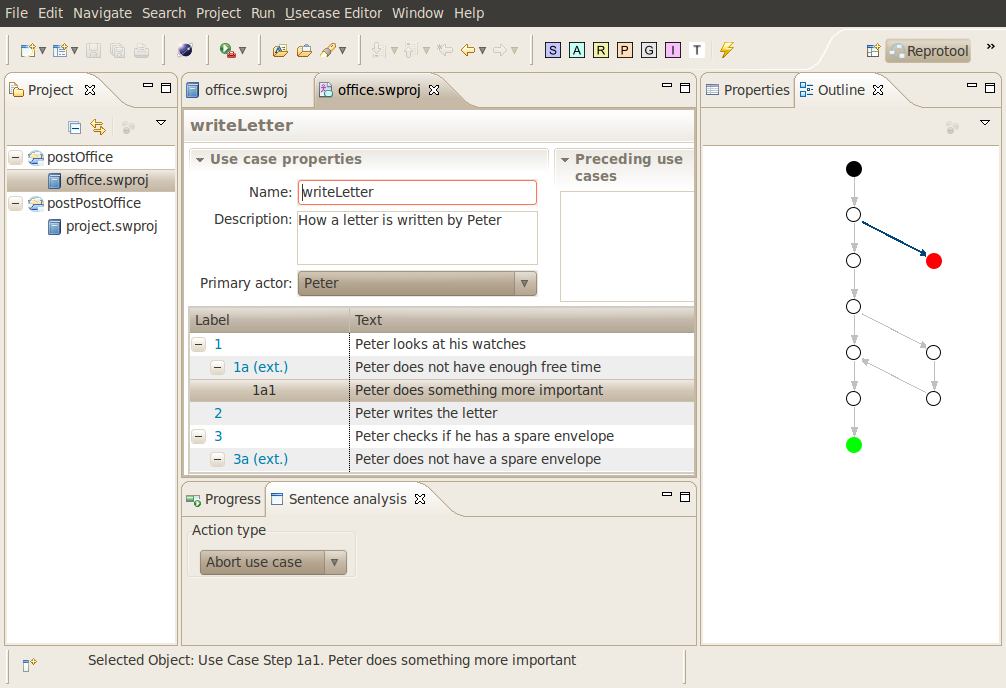
\includegraphics[height=280pt]{images/reprotoolAbort}
  \caption{\emph{Abort} use-case step action specified}
  \label{fig:reprotoolAbort}
\end{figure}

\newpage

Now we will define an \emph{include action} for the use-case step with label \emph{3a2}. So click this use-case step and in the
\emph{Analysis} view, select \emph{Use case include} as the action type and select the use-cese \emph{buyEnvelope} as the included
use-case. You can view the situation in the next picture. Also notice the outline view that shows also the included use-case schema. 

\begin{figure}[ht]
  \centering
  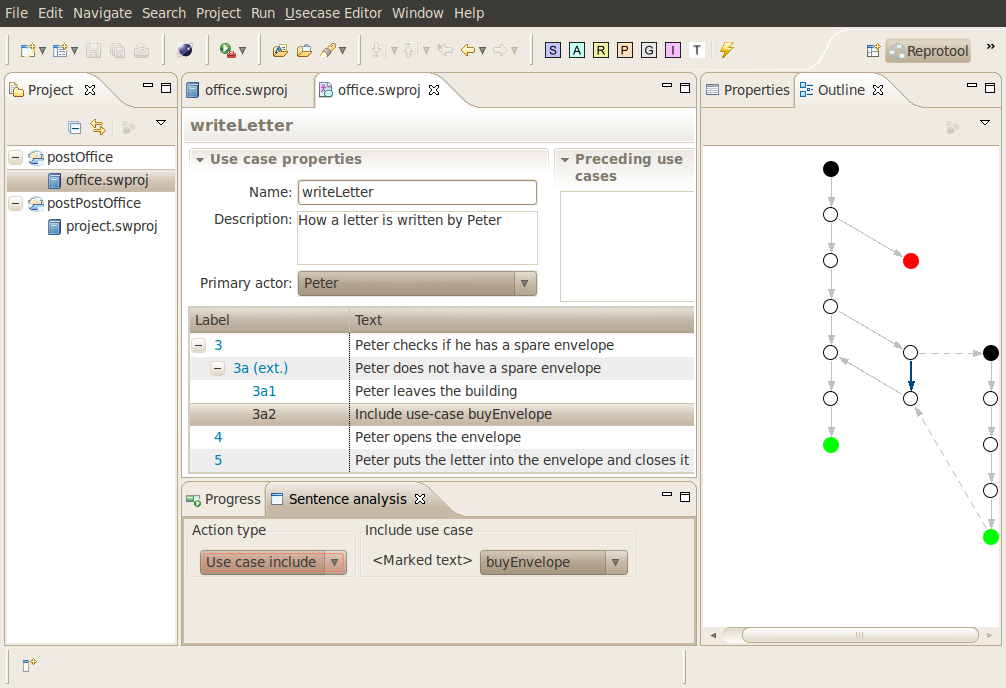
\includegraphics[height=280pt]{images/reprotoolInclude}
  \caption{\emph{Include} use-case step action specified}
  \label{fig:reprotoolInclude}
\end{figure}

\subsubsection{\emph{Actions} in the \emph{takeLetter} use-case}

Now, please specify the \emph{Abort} action for the use-case step labeled \emph{3a1} in the \emph{takeLetter} use-case. (The step text
reads: \emph{Peter goes home}).

\subsubsection{\emph{Actions} in the \emph{buyEnvelope} use-case}
There are no actions specified in this use-case.

\newpage

\subsection{Add \emph{annotations} to the use-case steps}

In this step we will need the \emph{Properties} view. If it is not displayed, you can show it with this command:
\begin{verbatim}
 Window / Show View / Properties
\end{verbatim}

Now we will add \emph{annotations} to some of the use-case steps. The newly created \emph{Reprotool} project already contains a vocabulary
of annotations that are ready to be used. We will now show how to use them.

\subsubsection{\emph{Annotations} in the \emph{writeLetter} use-case}
The second use-case step of this use-case reads: \emph{Peter writes the letter}. We will add an annotation of
type \emph{create} to this step. Right-click on this step in the use-case editor. Execute this command:
\begin{verbatim}
 New Child / StepAnnotation
\end{verbatim}
A new \emph{Annotation} will be created under the specified use-case step. Now look at the \emph{Properties view} and select
\emph{create} as annotation type. Write \emph{letter} as annotation id. Notice in the \emph{Properties view}, that \emph{Reprotool}
automatically generates an annotation \emph{description} by concatenating the annotaion \emph{type} and the annotation \emph{id}.
In this case it reads \emph{\#create\_letter}.
Also notice that in the \emph{OutlineView} the annotated use-case steps have a small violet square drawn over them. You can view this
situation in the next figure:

\newpage

\begin{figure}[ht]
  \centering
  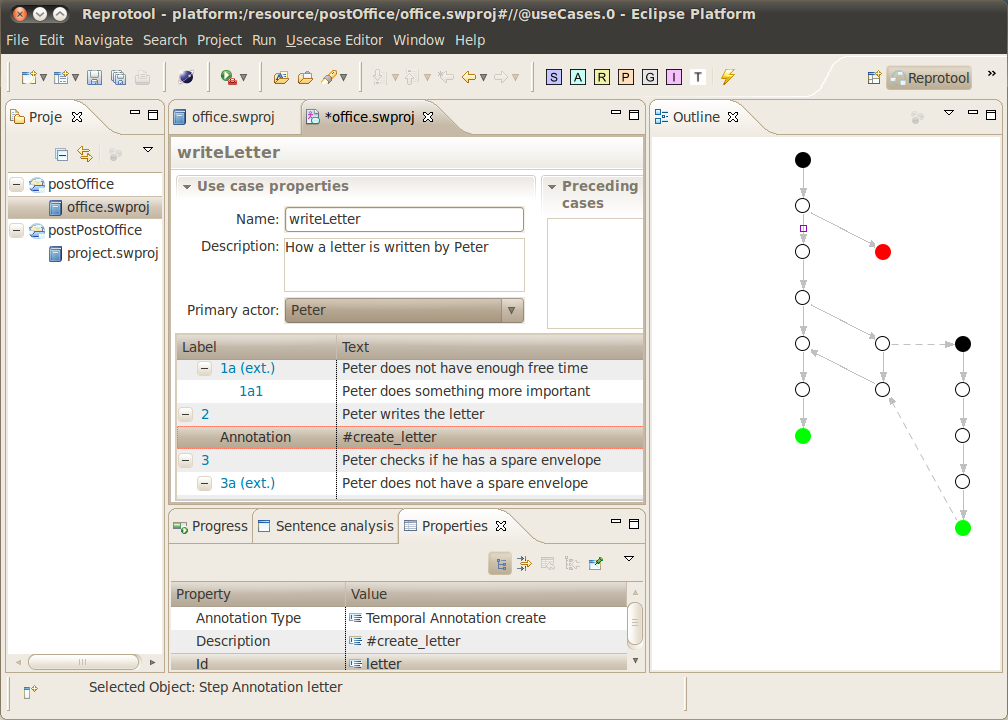
\includegraphics[height=280pt]{images/reprotoolAnnot}
  \caption{\emph{create} annotation specified}
  \label{fig:reprotoolAnnot}
\end{figure}

Now add the annotation \emph{\#open\_envelope} to the step \emph{Peter opens the envelope} and add annotation \emph{\#close\_envelope}
to the step \emph{Peter puts the letter into the envelope and closes it}.

\subsubsection{\emph{Annotations} in the \emph{takeLetter} use-case}
Please add the annotaion \emph{\#create\_letter} to the step in use-case \emph{takeLetter} that reads: \emph{Peter goes home}\footnote{Please don't be worried if you think this annotation does not belong here. Indeed, it doesn't. But we create it
here just to show in the later part of this tutorial what happens when you break the semantics of annotations.}.
Also add the annotaion \emph{\#use\_letter} to the step in the same use-case that reads: \emph{The post officer takes the letter
from Peter}.

\subsubsection{\emph{Annotations} in the \emph{buyEnvelope} use-case}
There are no annotations in this use-case.

\newpage

\subsection{Specify \emph{precedence relations} between use-cases.}

We will now add a precedence relation between use-cases \emph{writeLetter} and \emph{takeLetter} specifying that the use-case
\emph{takeLetter} can be executed only after the use-case \emph{writeLetter} successfully finished. Open now the use-case
\emph{takeLetter} in the use-case editor. Click on the icon in the \emph{Preceding use-cases} area. A dialog box now appears that
allows you to specify preceding use-cases of the use-case \emph{takeLetter}. Now select the \emph{writeLetter} use-case in the left part
of the dialog window and click the \emph{add} button to copy this use-case to the right part of the window. Then just press OK. This
situation is depicted in this figure:

\begin{figure}[ht]
  \centering
  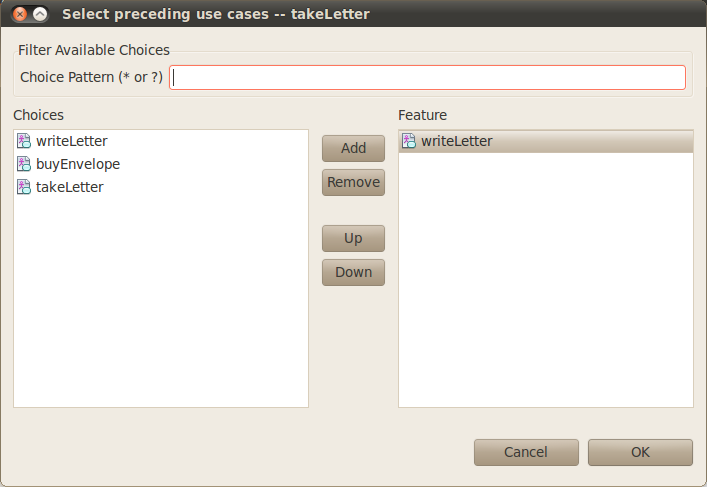
\includegraphics[height=280pt]{images/reprotoolPrecede}
  \caption{\emph{precede} annotation specified}
  \label{fig:reprotoolPrecede}
\end{figure}

\subsection{Keyboard shortcuts available in Project and Use case editor}

To speed up manipulation with objects in \emph{Reprotool} user can use these keyboard shortcuts:

\verb|Delete| removes selected \emph{Conceptual object}, \emph{Actor} or \emph{Use case} in \emph{Project editor}.
In \emph{Use case editor} it removes removes selected \emph{Use case step}, \emph{Annotation}, \emph{Extension} or \emph{Variation}.  

\verb|Ctrl + Enter| in \emph{Use case editor} adds new \emph{Use case step} after currently selected one.

\verb|Ctrl + 1| and \verb|Ctrl + 2| in \emph{Use case editor} adds new \emph{Extension} or \emph{Variation} of the selected use case step.

\verb|Ctrl + 4| in \emph{Use case editor} adds new \emph{Annotation} of the selected use case step.

